%------ setup ------

\documentclass[11pt, a4paper]{article}

% set margins
\usepackage[a4paper, margin=2.5cm]{geometry}

% use Times New Roman
\usepackage{mathptmx}
\usepackage[T1]{fontenc}

% double line spacing
\usepackage{setspace}
\doublespacing

% for justify
\usepackage{ragged2e}
\usepackage{fontspec}



% prevents hyphenation throughout the document.
\usepackage[none]{hyphenat}

% displaying images
\usepackage{graphicx}
\graphicspath{ {./images/} }

% use hungarian names for some of the text generated by packages (e.g. Table of Contents, Figure)
\usepackage[hungarian]{babel}

% for minipage captions inside items
\usepackage{caption}

% another option is to redefine commands, e.g.: Table of Contents to Tartalomjegyzék
% rename ToC
%\renewcommand{\contentsname}{Tartalomjegyzék}

% make ToC linkable
\usepackage[hidelinks]{hyperref}

% use begin{figure}[h] to place the image under the text

% for framing figures
\usepackage{framed}

% for sizing the tables
\usepackage{array}

% for using font colors
\usepackage[dvipsnames]{xcolor}

% for formatted code
\usepackage{listings}

\definecolor{eclipseStrings}{RGB}{42,0.0,255}
\definecolor{eclipseKeywords}{RGB}{127,0,85}
\colorlet{numb}{magenta!60!black}

\lstdefinelanguage{json}{
	basicstyle=\normalfont\ttfamily,
	commentstyle=\color{eclipseStrings}, % style of comment
	stringstyle=\color{eclipseKeywords}, % style of strings
	%numbers=left,
	%numberstyle=\scriptsize,
	stepnumber=0,
	numbersep=0pt,
	showstringspaces=true,
	breaklines=true,
	%frame=single,
	%backgroundcolor=\color{white}, %only if you like
	string=[s]{"}{"},
	comment=[l]{:\ "},
	morecomment=[l]{:"},
	tabsize=1,
	literate=
	*{0}{{{\color{numb}0}}}{1}
	{1}{{{\color{numb}1}}}{1}
	{2}{{{\color{numb}2}}}{1}
	{3}{{{\color{numb}3}}}{1}
	{4}{{{\color{numb}4}}}{1}
	{5}{{{\color{numb}5}}}{1}
	{6}{{{\color{numb}6}}}{1}
	{7}{{{\color{numb}7}}}{1}
	{8}{{{\color{numb}8}}}{1}
	{9}{{{\color{numb}9}}}{1}
}

% ------ start of the document ------
\begin{document}
	
	\begin{titlepage}
		\vspace*{\fill}
		\begin{center}
			\Huge \textbf{Fejlesztői dokumentáció} \\
			Vidics Márk \\
			T1YAAB \\
			Mérnökinformatikus BSc
		\end{center}
		\vspace*{\fill}
	\end{titlepage}
	
	\tableofcontents
	\listoftables
	
	\section{A projekt áttekintése}
		\subsection{Funkcionális követelmények}
			\begin{itemize}
			\justifying
				\item A projekt célja egy olyan bemutató berendezés elkészítse, amely segítségével képesek vagyunk belépési eseményeket megjeleníteni, illetve karbantartani RFID kulcsok segítség-\\ével.
				
				\item Szükségünk van egy kártyaolvasó eszközre, amely képes a felhasználóknak kiosztott kár-\\tyák/kulcsok értékét beolvasni.
				
				\item Képesnek kell lennünk ezeket a kártyákat felhasználókhoz társítanunk.
				
				\item A rendszernek meg kell tudnia jeleníteni egy felhasználó belépése során a belépés állapotát, amik a következőek lehetnek: engedélyezett, tiltott és nem ismert kártya.
				
				\item A rendszernek rendelkeznie kell egy szolgáltatással, aminek segítségével valamilyen hálózati csatornán keresztül (pl.: HTTP kérések által) lekérdezhetőek és karbantarthatóak az RFID kulcsok, a felhasználók és a belépések.
				
				\item Gondoskodnunk kell arról, hogy ha egy felhasználó több alkalommal tiltott kártyával lép be, akkor üzenetet küldjünk a szolgáltatást üzemeltető rendszergazdának.
			\end{itemize}
		\vfill
		\subsection{Nem funkcionális követelmények}
			\begin{itemize}
				\justifying
				\item Egy Raspberry Pi 4 Model B eszköz még a projekt tervezése előtt beszerzésre került, ezért ez nem jelent külön kiadást, így a projektet ezzel kell megvalósítanunk, mert elégséges funkciókkal rendelkezik mind hardveres, mint szoftveres szinten.
				
				\item Egy bemutató eszköz elkészüléséhez az elektronikai elemeket tekintve maximum 10.000 forint összegű keretet szabunk meg. Ez egyben azt is meghatározza, hogy milyen hardverek jöhetnek szóba.
			\end{itemize}
	\section{Tervezési fázis}
		\subsection{Hardveres tervek}
			\begin{itemize}
				\justifying
				
				\item A hardver elemek kiválasztása során figyelembe kell vennem, hogy a nem funkcionális követelményként meghatározott Raspberry Pi-hoz alkalmas eszközöket válasszak. Így ez esetben a GPIO lábkiosztása fogja nekünk megszabni azt, hogy pontosan milyen kommuni-\\kációs csatornán tudunk adatokat küldeni és fogadni. 
				
				\item Szükség esetén az adott integrált áramköri panelek (pl.: RFID olvasó) lábait a csatlakozási pontokhoz kell forrasztani, ezért a forrasztóállomás beszerzéséről és egyéb kellékekről is gondoskodni kell.
				
				\item A bemutató eszközt próba panelen célszerű elkészíteni, mert az adott bekötés könnyen módosítható, illetve nem kell forrasztási műveleteket sem végezni ehhez.
			\end{itemize}
		\subsection{Szoftveres tervek}
			\begin{itemize}
				\justifying
				\item A Raspberry Pi 4 Model B eszköz (lényegében egy ARM architektúrájú kis számítógépről van szó) rendelkezik a gyártó által fejlesztett operációs rendszerrel, ezért ennek használata tűnt a legcélszerűbbnek, mert könnyen kezelhető és széleskörű csomagtámogatással rendel-\\kezik.
				
				\item Követelményként szükségünk van egy adatokat szolgáltató alkalmazást fejleszteni, és mivel egy bemutató alkalmazásról van szó, ezért az egyszerűség kedvéért Python nyelven készül el, különböző \texttt{pip} csomagok használatával.
				
				\item Az adattároláshoz szükséges adatbázis kezelő kiválasztásánál is az egyszerűséget és könnyű kezelhetőséget érdemes alapul venni, ami esetén a MySQL jó választásnak bizonyul.
			\end{itemize}
	
	\section{Hardver specifikáció}			
		\subsection{Raspberry Pi}
		\begin{flushleft}
			\justifying
			Az eszköz rendelkezik egy 40 csatlakozási pontos GPIO interfésszel. Ennek van egy belső számozása, amit a Raspberry Pi rendszere tud kezelni, illetve egy 1-40-ig tartozó számsorozat, ami a teljes lábkiosztásra vonatkozik. A következő ábrán a \emph{GPIO\#} jelölés a belső számozást, a csatlakozási pontok melletti számok pedig a teljes lábkiosztást adják meg. Az LCD kijelző és az RFID olvasó a teljes lábkiosztás szerint van bekötve.
		\end{flushleft}
			\begin{minipage}{\linewidth}
				\centering
				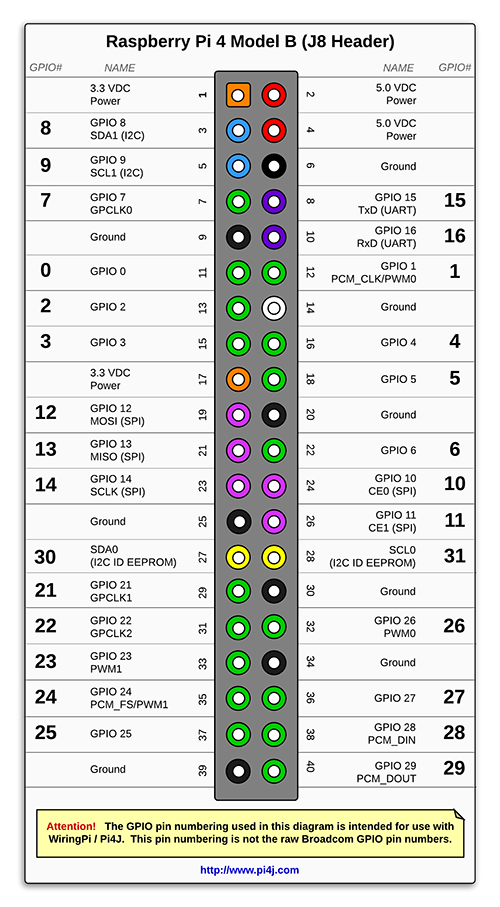
\includegraphics[width=0.6\linewidth]{img/rpi_pinout}
				\captionof{figure}{Raspberry Pi 4 Model B lábkiosztása}
				\label{fig:2rpipinout}
			\end{minipage}
			
		\subsection{RFID olvasó}
		\begin{flushleft}
			\justifying
			A felhasznált RFID olvasó modellje: RC522-MFRC. A kommunikáció az olvasóval SPI interfészen keresztül történik, melynek értékét ütemezett intervallumokban lekérdezzük és a táblázatban részletezett módon kerül bekötésre.
		\end{flushleft}
			\begin{minipage}{\linewidth}
				\centering
				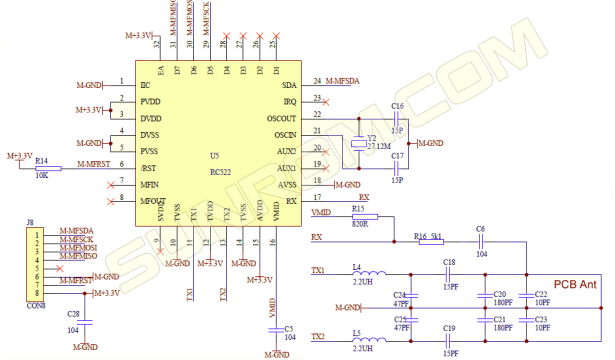
\includegraphics[width=0.7\linewidth]{img/rc552_shematic}
				\captionof{figure}{Az RFID olvasó kapcsolási rajza}
				\label{fig:3rfidschematic}
			\end{minipage}
			\begin{minipage}{\linewidth}
				\centering
				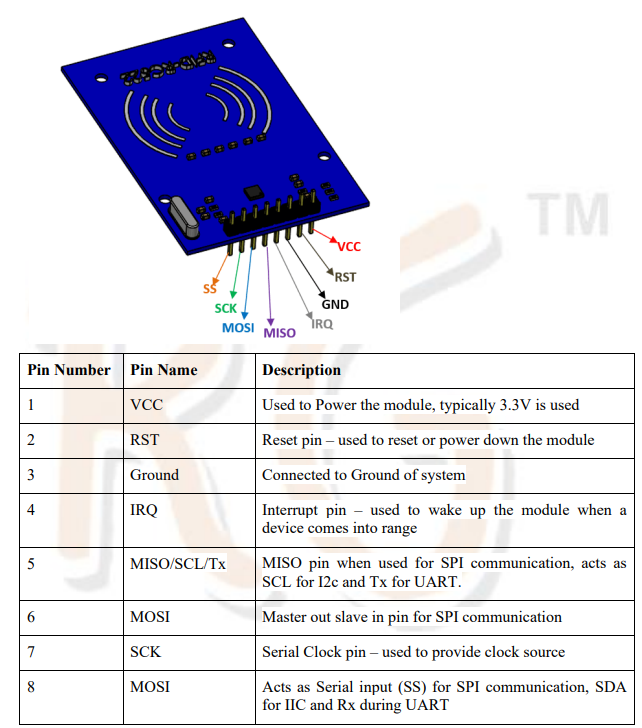
\includegraphics[width=0.7\linewidth]{img/rc552_pinout}
				\captionof{figure}{Az RFID olvasó lábkiosztása}
				\label{fig:4rfidpinout}
			\end{minipage}
			
			\begin{minipage}{\linewidth}
				\fontsize{10}{16}\selectfont
				\centering
				\begin{tabular}{||m{6em} m{6em}||}
					\hline
					\multicolumn{2}{|c|}{\textbf{RC522-MFRC olvasó bekötési terv}} \\
					\hline
					\texttt{Raspberry GPIO pin száma} & \texttt{RFID pin neve} \\
					\hline\hline
					17 & VCC \\ 
					\hline
					22 & RST \\ 
					\hline
					20 & GND \\ 
					\hline
					21 & MISO \\
					\hline
					19 & MOSI \\
					\hline
					23 & SCK \\
					\hline
					24 & SDA (MOSI) \\
					\hline
				\end{tabular}
				\captionof{table}{Az RFID olvasó bekötési terve}
				\label{table:rfidconnections}
			\end{minipage}
			
		\subsection{LCD kijelző}
		\begin{flushleft}
			\justifying
			A felhasznált LCD kijelző modellje: KC-1602-BB-I2C. A kommunikáció I$^2$C csomag-\\kapcsolt soros buszon keresztül történik és a táblázatban részletezett módon kerül bekötésre.
		\end{flushleft}
		\begin{minipage}{\linewidth}
			\centering
			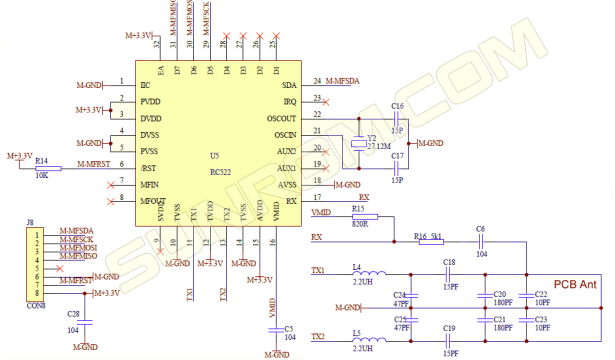
\includegraphics[width=1.0\linewidth]{img/rc552_shematic}
			\captionof{figure}{Az LCD olvasó kapcsolási rajza}
			\label{fig:4lcdshematic}
		\end{minipage}
		\begin{minipage}{\linewidth}
			\centering
			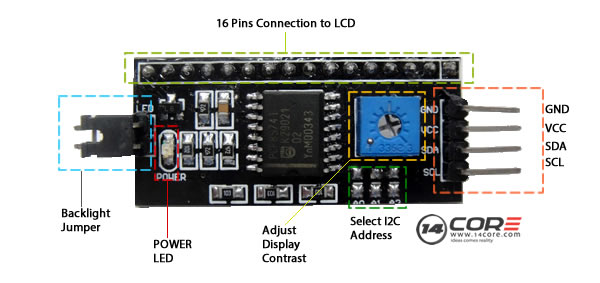
\includegraphics[width=1.0\linewidth]{img/i2c_pinout}
			\captionof{figure}{Az LCD kijelző kivezetési pontjai}
			\label{fig:5lcdpinout}
		\end{minipage}
		\begin{minipage}{0.5\linewidth}
			\fontsize{10}{16}\selectfont
			\centering
			\begin{tabular}{||m{6em} m{8em}||}
				\hline
				\multicolumn{2}{|c|}{\textbf{KC-1602-BB-I2C lábkiosztás}} \\
				\hline
				\texttt{Pin} & \texttt{Funkció} \\
				\hline\hline
				GND & Földelési pont \\ 
				\hline
				VCC & 5V tápellátás \\ 
				\hline
				SDA & Soros adatvonal \\ 
				\hline
				SCL & Soros órajel \\
				\hline
			\end{tabular}
			\captionof{table}{Az LCD kijelző felhasznált lábai}
			\label{table:lcdpinout}
		\end{minipage}
		\begin{minipage}{0.5\linewidth }
			\fontsize{10}{16}\selectfont
			\centering
			\begin{tabular}{||m{6em} m{8em}||}
				\hline
				\multicolumn{2}{|c|}{\textbf{KC-1602-BB-I2C bekötési terv}} \\
				\hline
				\texttt{Raspberry GPIO pin száma} & \texttt{RFID pin neve} \\
				\hline\hline
				9 & GND \\ 
				\hline
				2 & VCC \\ 
				\hline
				3 & SDA \\ 
				\hline
				5 & SCL \\
				\hline
			\end{tabular}
			\captionof{table}{Az LCD kijelző bekötési terve}
			\label{table:lcdconnections}
		\end{minipage}
		\subsection{Próbapanel}
			A felhasznált próbapanel modellje: BB-102 (630/200) \\
		\begin{minipage}{\linewidth}
			\centering
			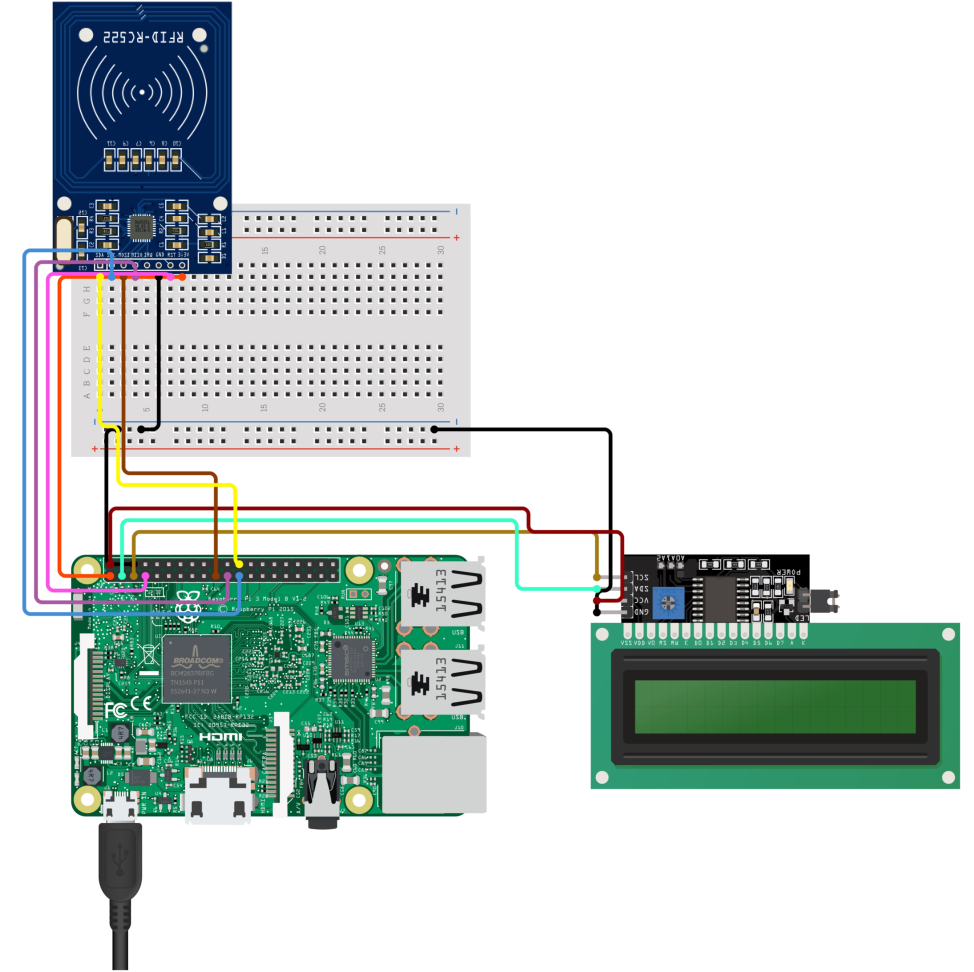
\includegraphics[width=0.7\linewidth]{img/breadboard_diagram}
			\captionof{figure}{A hardveres terv próbapanelen}
			\label{fig:1breadboarddiagram}
		\end{minipage}
		\begin{minipage}{\linewidth}
			\centering
			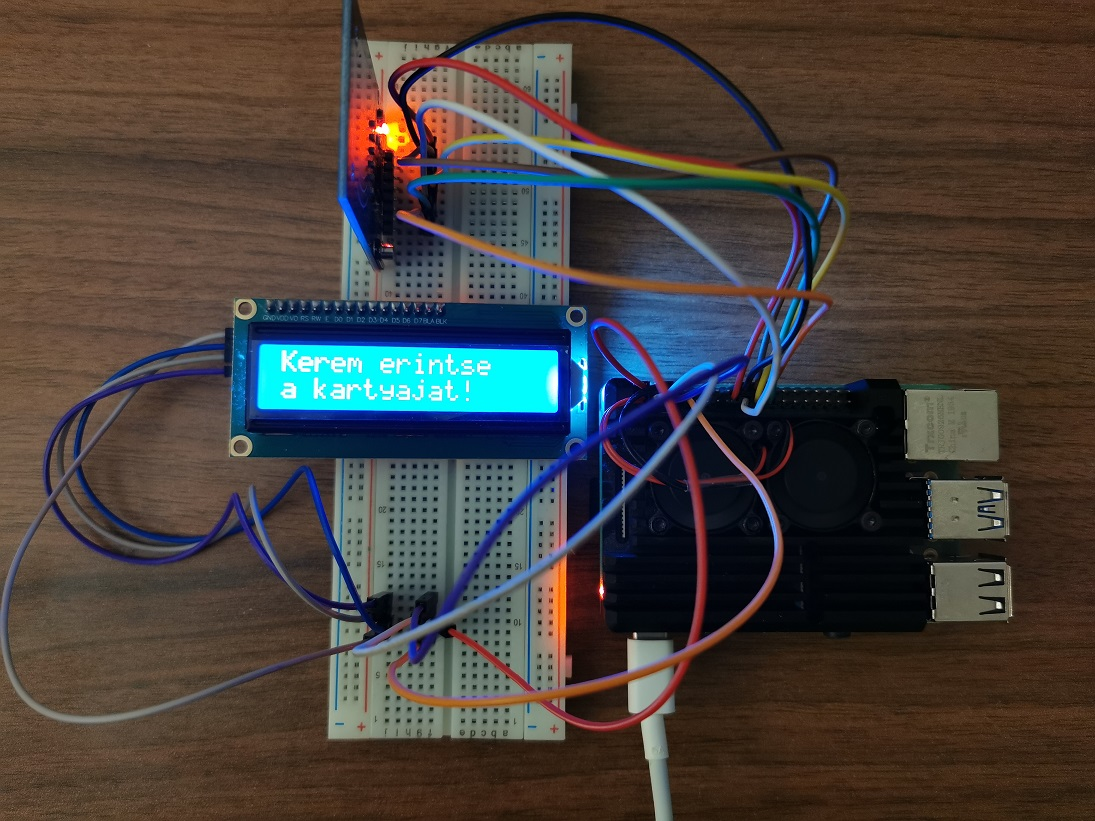
\includegraphics[width=0.7\linewidth]{img/3_futas}
			\captionof{figure}{A projekt tényleges megvalósítása üzemkész állapotban}
			\label{fig:3futas}
		\end{minipage}
		
	\section{Szoftver specifikáció}
		\subsection{Raspberry Pi OS}
			\begin{flushleft}
				\justifying
				A Raspberry Pi OS egy Debian alapú operációs rendszer, ami kifejezetten a Raspberry Pi hardverekhez lett létrehozva, így ez már tartalmazza a szükséges rendszerszintű függvénykönyv-\\tárakat ahhoz, hogy a hardveres kommunikációt meg tudjuk valósítani. A gyártó által készített függvénykönyvtárakat számos közösségi és egyéni fejlesztő által létrehozott csomag felhasználja, aminek segítségével képesek vagyunk absztraktabb szinten is kommunikálni ezekkel a hardveres eszközökkel, például Python nyelven. A következő operáció rendszer van telepítve:
				\begin{itemize}
					\item Kiadási dátum: 2023 október 10.
					\item Rendszer: 64-bit
					\item Kernel verzió: 6.1
					\item Debian verzió: 12 (bookworm)
				\end{itemize}

			\end{flushleft}
		\subsubsection{Docker}
			\begin{flushleft}
				\justifying
				A Docker egy konténeres virtualizációs platform, lehetővé teszi a felhasználóknak, hogy szoftver-\\alkalmazásokat izolált környezetben futtassák. A konténereket könnyedén és gyorsan el lehet indítani, amik általában egy \emph{Dockerfile} alapján vannak definiálva. A konténerben futott szoftver alapját az úgy nevezett \emph{base image} adja meg. Ebben az esetben ez a megoldás a MySQL adatbázis kezelő szoftverhez van használva, mert így el lehet kerülni a telepítési nehézségeket, valamint a konténert bármikor le tudjuk állítani vagy el tudjuk indítani. A konténer indítását a jelenlegi projekt esetén a szolgáltatáshoz tartozó indító szkript rendszerindításkor megteszi.
			\end{flushleft}

	\section{A fejlesztett kód részletezése}
		\subsection{Adatbázis szerkezet}
			\begin{flushleft}
				\justifying
				A szolgáltatás mögött egy MySQL adatbázis fut a korábban említett Docker konténerben, ami a belépési idők rögzítését, illetve az adott felhasználóhoz tartozó belépési idők lekérdezését hívatott megvalósítani. Az adatbázis szerkezete a következő ábrán és táblázatokon van részletezve: \\
			\end{flushleft}
			\begin{minipage}{\linewidth}
				\centering
				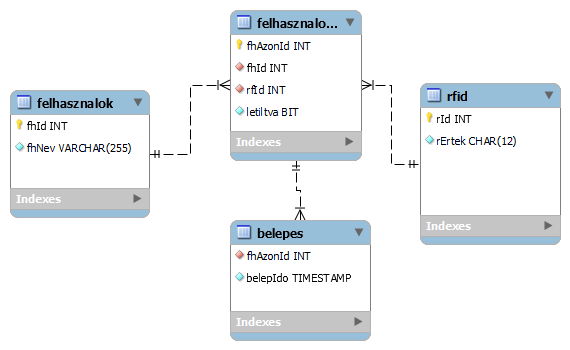
\includegraphics[width=0.9\linewidth]{../db/db_diagram}
				\captionof{figure}{Egyed-kapcsolat modell}
				\label{fig:dbdiagram}
			\end{minipage}
			\vfill
				\begin{minipage}{\linewidth}
					\fontsize{10}{16}\selectfont
					\centering
					\begin{tabular}{||m{6em} m{6.5em} m{10em} m{12em}||}
						\hline
						\multicolumn{4}{|c|}{\textbf{Felhasznalok}} \\
						\hline
						\texttt{Oszlop név} & \texttt{Típus} & \texttt{Tulajdonságok} & \texttt{Funkció} \\ 
						\hline\hline
						fhId & INT & UNIQUE NOT NULL AUTO\_INCREMENT & A felhasználó azonosítója \\ 
						\hline
						fhNev & VARCHAR(255) & NOT NULL & A felhasználó neve \\
						\hline
					\end{tabular}
					\captionof{table}{Az felhasználókkal kapcsolatos alapinformációk tárolása}
					\label{table:1}
				\end{minipage}
				\vfill
				
				\begin{minipage}{\linewidth}
					\fontsize{10}{16}\selectfont
					\centering
					\begin{tabular}{||m{6em} m{6em} m{10em} m{12em}||}
						\hline
						\multicolumn{4}{|c|}{\textbf{Rfid}} \\
						\hline
						\texttt{Oszlop név} & \texttt{Típus} & \texttt{Tulajdonságok} & \texttt{Funkció} \\
						\hline\hline
						rId & INT & UNIQUE NOT NULL AUTO\_INCREMENT & Az RFID azonosítója \\ 
						\hline
						rErtek & CHAR(12) & UNIQUE NOT NULL & Az RFID kulcs értéke \\ 
						\hline
					\end{tabular}
					\captionof{table}{Az RFID kulccsal kapcsolatos alapinformációk tárolása}
					\label{table:2}
				\end{minipage}
				\vfill
	
				\begin{minipage}{\linewidth}
					\fontsize{10}{16}\selectfont
					\centering
					\begin{tabular}{||m{6em} m{6em} m{10em} m{12em}||}
						\hline
						\multicolumn{4}{|c|}{\textbf{FelhasznaloAzonosito}} \\
						\hline
						\texttt{Oszlop név} & \texttt{Típus} & \texttt{Tulajdonságok} & \texttt{Funkció} \\
						\hline\hline
						fhAzonId & INT & UNIQUE NOT NULL AUTO\_INCREMENT & Egy rekord azonosítója \\ 
						\hline
						fhId & INT & NOT NULL & A felhasznalok tábla fhId oszlopa \\ 
						\hline
						rId & CHAR(12) & UNIQUE NOT NULL & Az RFID tábla rId oszlopa \\ 
						\hline
						letiltva & BIT & NOT NULL DEFAULT 0 & A felhasználóhoz rendelt RFID azonosító tiltásának állapota \\
						\hline
					\end{tabular}
					\captionof{table}{Egy felhasználó összekapcsolása több RFID kulccsal (egy-a-többhöz)}
					\label{table:3}
				\end{minipage}
				\vfill
				
				\begin{minipage}{\linewidth}
					\fontsize{10}{16}\selectfont
					\centering
					\begin{tabular}{||m{6em} m{6em} m{12.5em} m{12em}||}
						\hline
						\multicolumn{4}{|c|}{\textbf{Belepes}} \\
						\hline
						\texttt{Oszlop név} & \texttt{Típus} & \texttt{Tulajdonságok} & \texttt{Funkció} \\
						\hline\hline
						fhAzonId & INT & NOT NULL & A felhasznaloAzonosito fhAzonId oszlopa \\ 
						\hline
						belepIdo & TIMESTAMP & NOT NULL\newline{} DEFAULT CURRENT\_TIMESTAMP() & A belépés ideje \\ 
						\hline
						rId & CHAR(12) & UNIQUE NOT NULL & Az RFID tábla rId oszlopa \\ 
						\hline
						letiltva & BIT & NOT NULL DEFAULT 0 & A felhasználóhoz rendelt RFID azonosító tiltásának állapota \\
						\hline
					\end{tabular}
					\captionof{table}{Egy felhasználóhoz tartozó RFID kulcs belépési idejének tárolása}
					\label{table:4}
				\end{minipage}
			
		\subsection{Verziókövető rendszer}
			\begin{flushleft}
				\justifying
				A projekt követelményeknek megfelelően a kód GitHubon van tárolva, ami
				 \color{blue}
				 \href{https://github.com/mark182182/GKLB_INTM020_mikroelektromechanikai_rendszerek}{ezen a linken elérhető}\color{black}.
			\end{flushleft}
			
		\subsection{Konfiguráció}
			\begin{flushleft}
				\justifying
				Az alkalmazásban használt beállításokat egy
				\color{blue} \href{https://github.com/mark182182/GKLB_INTM020_mikroelektromechanikai_rendszerek/blob/main/config.ini}{config.ini}
				\color{black}
				fájlból olvassuk ki. A Pythonban képesek vagyunk a \texttt{configparser} csomag segítségével egy előre megadott struktúrában definiálni kulcs-\\érték párokat. Ezeket az értékeket kétféle módon használjuk fel: egy az egyben olvassuk ki, vagy érzékeny adatok esetén mutathat egy környezeti változóra is, például ilyen az adatbázis jelszó. Így meggátolhatjuk azt, hogy ezek az adatok a távoli verziókövető rendszerbe legyenek feltöltve, valamint elérjük vele azt is, hogy kizárólag az adott környezetben beállított változókkal tudjanak működni.\\
				A felhasználásuk a következő módon történik:
				\begin{itemize}
					\item \texttt{[mysql]} alatt:
					\begin{itemize}
						\item Host: A MySQL adatbázis IP címe
						\item User: A MySQL adatbázishoz tartozó felhasználó
						\item Password: A MySQL adatbázishoz tartozó jelszó
						\item Database: A MySQL adatbázishoz neve
					\end{itemize}
					\item \texttt{[smtp]} alatt:
						\begin{itemize}
							\item Host: A SMTP szerver címe
							\item Port: A SMTP szerverhez tartozó port
							\item User: A SMTP szerverhez szükséges felhasználó
							\item Password: A SMTP szerverhez szükséges jelszó
							\item FromAddress: Az emailt küldő címe
							\item ToAddress: Az emailt fogadó címe
							\item DebugLevel: Logikai változó, amely segítségével extra információt kapunk az SMTP szerverrel való kommunikációról
						\end{itemize}
				\end{itemize}
				Dokumentáció a \texttt{configparser} csomagról
				\color{blue}
				\href{https://docs.python.org/3/library/configparser.html}{ezen a linken elérhető}\color{black}.
			\end{flushleft}
			
		\subsection{Indító szkript}
			\begin{flushleft}
				\justifying
				Az implementáció a következő fájlban található:
				\color{blue}
				\href{https://github.com/mark182182/GKLB_INTM020_mikroelektromechanikai_rendszerek/blob/main/start.sh}{start.sh}\\
				\color{black}
				A kódbázis tartalmát egy Python \texttt{venv} virtuális környezetben tároljuk. Ennek segítségével a futtatási környezetet izolálni tudjuk és az ebben található Python és egyéb binárisok segítéségével futtathatjuk a kódot. A letöltött csomagok csak erre a virtuális környezetre lesznek hatással, rendszerszinten nem települnek fel, így meggátolható az is, hogy a különböző verziójú binárisok összeakadjanak a Python ökoszisztémában. \\
				A szkript a következő fő lépésekre bontható:
				\begin{enumerate}
					\item Az indító szkript először leellenőrzi, hogy az említett virtuális környezeten belül használt binárisok léteznek-e.
					\item Ez után a
					\color{blue} \href{https://github.com/mark182182/GKLB_INTM020_mikroelektromechanikai_rendszerek/blob/main/requirements.txt}{requirements.txt}
					\color{black} fájlból feltelepíti az abban definiált csomagokat a \texttt{pip} csomag-\\kezelő segítségével.
					\item Következő lépésben a virtuális környezetben elhelyezett \texttt{.env} fájlból beállítjuk az érzékeny adatokhoz tartozó környezeti változókat.
					\item Következőnek elindítjuk az adatbázist tartalmazó és működtető Docker konténert, illetve ez létrehozása kerül, ha még korábban nem volt elkészítve.
					\item Végső soron elindítjuk a szolgáltatást a \texttt{flask} segítségével. Ez a csomag később, az \ref{subs:httpcalls} részen kerül bemutatásra.
				\end{enumerate}
				Információ a Python \texttt{venv} modulról
				\color{blue}
				\href{https://docs.python.org/3/library/venv.html}{ezen a linken elérhető}\color{black}.\\
				Információ a Python \texttt{pip} csomagkezelőről
				\color{blue}
				\href{https://pip.pypa.io/en/stable/user_guide/}{ezen a linken elérhető}\color{black}.
			\end{flushleft}

		\subsection{Adatbáziskapcsolat}
			\begin{flushleft}
				\justifying
				A szolgáltatásban az adatbáziskapcsolatot a \texttt{mysql-connector-python} csomag segítségével hajt-\\ja végre a
				\color{blue}
				\href{https://github.com/mark182182/GKLB_INTM020_mikroelektromechanikai_rendszerek/blob/main/db/db.py}{db.py}
				\color{black} fájl. A kapcsolatra annak sikeres létrehozása után, az osztályban eltárolt \texttt{conn} adattaggal tudunk később hivatkozni. A kapcsolat létrejöttekor az adatbázist elkészítjük, (ha már létezik, akkor töröljük és újra létrehozzuk) majd példa adatokkal töltjük fel a \\ \color{blue}
				\href{https://github.com/mark182182/GKLB_INTM020_mikroelektromechanikai_rendszerek/blob/main/db/create_db_with_sample_data.sql}{create\_db\_with\_sample\_data.sql}
				\color{black} fájlban, azért, hogy a rendszer alapból rendelkezzen néhány felhasználóval, RFID-val, amihez a bemutatóban használt létező kulcsokat rendeltünk hozzá. Így a példában mind a három belépési állapotot le tudjuk fedni (letiltott, engedélyezett, a kártya nem létezik). \\
				Az adatbázis lekérdezésekhez szükséges kód a 
				\color{blue}
				\href{https://github.com/mark182182/GKLB_INTM020_mikroelektromechanikai_rendszerek/tree/main/repo}{repo}
				\color{black} mappában került megvalósításra.
			\end{flushleft}

		\subsection{SPI kommunikáció}
			\begin{flushleft}
				\justifying
				Az implementáció a következő fájlban található:
				\color{blue}
				\href{https://github.com/mark182182/GKLB_INTM020_mikroelektromechanikai_rendszerek/blob/main/raspi/rfid_spi.py}{rfid\_spi.py}
				\color{black} \\
				A kommunikáció a \texttt{pi-rc522} csomag segítségével történik, amely rendelkezik olyan tagfügg-\\vényekkel, ami az RFID olvasó aktuális állapotát le tudja kérdezni és karakterláncként visszaadni.
				A Python beépített \texttt{threading} moduljával képesek vagyunk időzítőt létrehozni, amely ez esetben másodpercenként kiolvassa az RFID olvasó aktuális értékét. Ha nem üres karakterláncot kapunk vissza az olvasótól, akkor továbbmegyünk az azonosítás részhez. \\
				Információ a Python \texttt{threading} modulról
				\color{blue}
				\href{https://docs.python.org/3/library/threading.html}{ezen a linken elérhető}\color{black}. \\
				Információ a \texttt{pi-rc522} csomagról
				\color{blue}
				\href{https://github.com/ondryaso/pi-rc522}{ezen a linken elérhető}\color{black}.
			\end{flushleft}
			
		\subsection{I$^2$C kommunikáció}
			\begin{flushleft}
				\justifying
				Az implementáció a következő fájlban található:
				\color{blue} \href{https://github.com/mark182182/GKLB_INTM020_mikroelektromechanikai_rendszerek/blob/main/raspi/lcd_i2c.py}{lcd\_i2c.py}
				\color{black} \\
				Az LCD kijelzővel való kommunikáció az \texttt{rpi\_lcd} csomag segítségével valósul meg. Alapértel-\\mezetten a \emph{Kerem erintse a kartyajat!} feliratot jelenítjük meg, majd kiírás során figyelünk arra, hogy a megjelenítendő üzenetet 5 másodpercig hagyjuk a kijelzőn, majd töröljük a tartalmat és visszaállítjuk az alapméretezett üzenetet. \\
				Információ az \texttt{rpi\_lcd} csomagról
				\color{blue}
				\href{https://github.com/bogdal/rpi-lcd}{ezen a linken elérhető}\color{black}.
				
			\end{flushleft}
		
		\subsection{Email küldés}
		\begin{flushleft}
			\justifying
			Az implementáció a következő fájlban található:
			\color{blue} \href{https://github.com/mark182182/GKLB_INTM020_mikroelektromechanikai_rendszerek/blob/main/smtp/smtp_client.py}{smtp\_client.py}
			\color{black} \\
			A kommunikáció az SMTP szerverrel az \texttt{smtplib} modul segítségével kerül megvalósításra. A szolgáltatás indításakor autentikáljuk a korábban említett konfigurációban megadott felhasználót. Abban az esetben, hogy ha a letiltott kártyák belépésének száma eléri a beállított értéket, (jelen esetben ez 3) akkor emailt küldünk a konfigurációban beállított címzettnek. A tartalom a \texttt{jinja2} csomag felhasználásával, az
			\color{blue}
			\href{https://github.com/mark182182/GKLB_INTM020_mikroelektromechanikai_rendszerek/blob/main/templates/unauthorized.html}{unauthorized.html}
			\color{black} minta segítségével jön létre. Ebben az emailben megjelenítjük a felhasználó azonosítóját, az RFID kártya számát és a tiltott kártyával történt belépési időket. \\
			Információ az \texttt{smtplib} modulról
			\color{blue}
			\href{https://docs.python.org/3/library/smtplib.html}{ezen a linken elérhető}\color{black}. \\
			Információ a \texttt{jinja2} csomagról
			\color{blue}
			\href{https://jinja.palletsprojects.com/en/3.1.x/}{ezen a linken elérhető}\color{black}.
		\end{flushleft}	
			
			
		\subsection{HTTP hívások}
			\label{subs:httpcalls}
			\begin{flushleft}
				\justifying
				A HTTP kérések kiszolgáláshoz szükséges kód a 
				\color{blue}
				\href{https://github.com/mark182182/GKLB_INTM020_mikroelektromechanikai_rendszerek/tree/main/route}{route}
				\color{black} mappában került megvalósításra. \\
				A különböző HTTP végpontok megvalósítását a \texttt{flask} csomag nyújtja, ami egy webalkalmazások fejlesztésére szolgáló keretrendszer, amely támogatja a \emph{Web Server Gateway Interface} (WSGI) szabványt.
				A válaszban visszaadott adatátviteli objektumok (DTO) a
				\color{blue}
				\href{https://github.com/mark182182/GKLB_INTM020_mikroelektromechanikai_rendszerek/tree/main/dto}{dto}
				\color{black} mappában vannak létrehozva. Ezek egyszerű objektumok, amelyek adatok tárolására, lekérdezésére, szerializálására és deszerializálására lettek létrehozva. Ezek segítségével pontosan annyi információt tudunk visszaadni, amennyire a kliensnek szüksége van. A kérések és válaszok esetén történő adatcserére a szövegalapú \texttt{JSON} szabványt használjuk. \\
				Információ a \texttt{flask} csomagról
				\color{blue}
				\href{https://flask.palletsprojects.com/en/3.0.x/}{ezen a linken elérhető}
				\color{black}.
			\end{flushleft}
			\subsubsection{Az implementált végpontok részletezése:}
				\begin{minipage}{\textwidth}
					\fontsize{6}{8}\selectfont
					\centering
					\begin{tabular}{|m{15em} | m{12em} | m{20em} | m{12em}|}
					\hline
					\multicolumn{4}{|c|}{\textbf{Felhasználók karbantartásához tartozó végpontok}} \\
					\hline
					\texttt{Végpont \newline{} (helyi hálózaton)} & \texttt{Minta JSON kérés} & \texttt{Sikeres válasz} & \texttt{Funkció} \\
					\hline
					GET http://localhost:5000/users &  &
					\fontsize{6}{2}\selectfont \begin{lstlisting}[language=json]
[
	{
		"py/object": "dao.user_dao.User",
		"_User__fhId": 1,
		"_User__fhNev": "Gipsz Jakab"
	},
	{
		"py/object": "dao.user_dao.User",
		"_User__fhId": 2,
		"_User__fhNev": "Nagy Paszkál"
	},
	{
		"py/object": "dao.user_dao.User",
		"_User__fhId": 3,
		"_User__fhNev": "Kiss Béla"
	}
]
					\end{lstlisting}
					& Az összes felhasználó lekérdezése \\
					\hline
					GET http://localhost:5000/user/3 &  &
\fontsize{6}{2}\selectfont \begin{lstlisting}[language=json]
{
	"py/object": "dao.user_dao.User",
	"_User__fhId": 3,
	"_User__fhNev": "Kiss Béla"
}
\end{lstlisting}
					& Egy megadott felhasználó lekérdezése azonosító alapján \\
					\hline
					DELETE http://localhost:5000/user/3 &  & success
& Egy megadott felhasználó törlése azonosító alapján \\
					\hline
					POST http://localhost:5000/user &
\fontsize{6}{2}\selectfont \begin{lstlisting}[language=json]
{
	"nev": "Teszt Béla"
}
\end{lstlisting}
					&
\fontsize{6}{2}\selectfont \begin{lstlisting}[language=json]
{
	"py/object": "dao.user_dao.User",
	"_User__fhId": 4,
	"_User__fhNev": "Teszt Béla"
}
\end{lstlisting}
& Egy felhasználó létrehozása név alapján \\
					\hline
					PATCH http://localhost:5000/user &
\fontsize{6}{2}\selectfont \begin{lstlisting}[language=json]
{
	"id": "2",
	"nev": "Teszt Csaba"
}
\end{lstlisting}
&
\fontsize{6}{2}\selectfont \begin{lstlisting}[language=json]
{
	"py/object": "dao.user_dao.User",
	"_User__fhId": 2,
	"_User__fhNev": "Teszt Csaba"
}
\end{lstlisting}
& Egy felhasználó nevének frissítése azonosító alapján \\
					\hline
					\end{tabular}
					\captionof{table}{A felhasználók karbantartásához tartozó végpontok}
					\label{table:5}
				\end{minipage}
				\begin{minipage}{\linewidth}
	\fontsize{6}{8}\selectfont
	\centering
	\begin{tabular}{|m{20em} | m{12em} | m{20em} | m{10em}|}
		\hline
		\multicolumn{4}{|c|}{\textbf{RFID karbantartásához tartozó végpontok}} \\
		\hline
		\texttt{Végpont \newline{} (helyi hálózaton)} & \texttt{Minta JSON kérés} & \texttt{Sikeres válasz} & \texttt{Funkció} \\
		\hline
		GET \newline{} http://localhost:5000/rfids &  &
		\fontsize{6}{2}\selectfont \begin{lstlisting}[language=json]
[
	{
		"py/object": "dao.rfid_dao.Rfid",
		"_Rfid__rId": 2,
		"_Rfid__rErtek": "1913502801"
	},
	{
		"py/object": "dao.rfid_dao.Rfid",
		"_Rfid__rId": 1,
		"_Rfid__rErtek": "3100821010"
	}
]
		\end{lstlisting}
		& Az összes RFID kulcs lekérdezése \\
		\hline
		GET \newline{} http://localhost:5000/rfid/3100821010 &  &
		\fontsize{6}{2}\selectfont \begin{lstlisting}[language=json]
{
	"py/object": "dao.rfid_dao.Rfid",
	"_Rfid__rId": 1,
	"_Rfid__rErtek": "3100821010"
}
		\end{lstlisting}
		& Egy megadott RFID lekérdezése azonosító alapján \\
		\hline
		DELETE \newline{} http://localhost:5000/rfid/3100821010 &  & success
		& Egy megadott RFID törlése azonosító alapján \\
		\hline
		POST \newline{} http://localhost:5000/rfid &
		\fontsize{6}{2}\selectfont \begin{lstlisting}[language=json]
{
	"ertek": "12345678"
}
		\end{lstlisting}
		&
		\fontsize{6}{2}\selectfont \begin{lstlisting}[language=json]
{
	"py/object": "dao.rfid_dao.Rfid",
	"_Rfid__rId": 10,
	"_Rfid__rErtek": "12345678"
}
		\end{lstlisting}
		& Egy RFID létrehozása érték alapján \\
		\hline
		PATCH \newline{} http://localhost:5000/rfid &
		\fontsize{6}{2}\selectfont \begin{lstlisting}[language=json]
{
	"id": "3",
	"ertek": "12345678"
}
		\end{lstlisting}
		&
		\fontsize{6}{2}\selectfont \begin{lstlisting}[language=json]
{
	"py/object": "dao.rfid_dao.Rfid",
	"_Rfid__rId": 3,
	"_Rfid__rErtek": "12345678"
}
		\end{lstlisting}
		& Egy RFID értékének frissítése azonosító alapján \\
		\hline
	\end{tabular}
	\captionof{table}{A RFID karbantartásához tartozó végpontok}
	\label{table:6}
\end{minipage}
\begin{minipage}{\linewidth}
	\fontsize{6}{8}\selectfont
	\centering
	\begin{tabular}{|m{20em} | m{12em} | m{23em} | m{10em}|}
		\hline
		\multicolumn{4}{|c|}{\textbf{Felhasználó és RFID kapcsolat karbantartásához tartozó végpontok}} \\
		\hline
		\texttt{Végpont \newline{} (helyi hálózaton)} & \texttt{Minta JSON kérés} & \texttt{Sikeres válasz} & \texttt{Funkció} \\
		\hline
		GET \newline{} http://localhost:5000/userId/2 &  &
		\fontsize{6}{2}\selectfont \begin{lstlisting}[language=json]
[
	{
		"py/object": "dao.user_id_dao.UserId",
		"_UserId__fhAzonId": 2,
		"_UserId__fhId": 2,
		"_UserId__rId": 2,
		"_UserId__rfErtek": "1913502801",
		"_UserId__letiltva": true
	}
]
		\end{lstlisting}
		& Egy felhasználóhoz tartozó RFID kulcsok lekérdezése felhasználó azonosító alapján \\
		\hline
		DELETE \newline{} http://localhost:5000/userId/12345678 &  & success
		& Egy felhasználóhoz tartozó RFID törlése RFID érték alapján \\
		\hline
		POST \newline{} http://localhost:5000/userId &
		\fontsize{6}{2}\selectfont \begin{lstlisting}[language=json]
{
	"fhId": "4",
	"rErtek": "12345678"
}
		\end{lstlisting}
		&
		\fontsize{6}{2}\selectfont \begin{lstlisting}[language=json]
{
	"py/object": "dao.user_id_dao.UserId",
	"_UserId__fhAzonId": 8,
	"_UserId__fhId": 4,
	"_UserId__rId": 3,
	"_UserId__rfErtek": "12345678",
	"_UserId__letiltva": false
}
		\end{lstlisting}
		& Egy RFID érték felhasználóhoz rendelése felhasználó azonosító alapján \\
		\hline
		PATCH \newline{} http://localhost:5000/userId/lock/1 &
		\fontsize{6}{2}\selectfont \begin{lstlisting}[language=json]
{
	"fhId": "4",
	"rId": "3"
}
		\end{lstlisting}
		&
		\fontsize{6}{2}\selectfont \begin{lstlisting}[language=json]
{
	"py/object": "dao.user_id_dao.UserId",
	"_UserId__fhAzonId": 8,
	"_UserId__fhId": 4,
	"_UserId__rId": 3,
	"_UserId__rfErtek": "12345678",
	"_UserId__letiltva": true
}
		\end{lstlisting}
		& Egy felhasználóhoz tartozó RFID kulcs tiltása azonosító alapján \\
		\hline
		PATCH \newline{} http://localhost:5000/userId/lock/0 &
\fontsize{6}{2}\selectfont \begin{lstlisting}[language=json]
{
	"fhId": "4",
	"rId": "3"
}
\end{lstlisting}
&
\fontsize{6}{2}\selectfont \begin{lstlisting}[language=json]
{
	"py/object": "dao.user_id_dao.UserId",
	"_UserId__fhAzonId": 8,
	"_UserId__fhId": 4,
	"_UserId__rId": 3,
	"_UserId__rfErtek": "12345678",
	"_UserId__letiltva": false
}
\end{lstlisting}
& Egy felhasználóhoz tartozó RFID kulcs engedélyezése azonosító alapján \\
\hline
	\end{tabular}
	\captionof{table}{A felhasználókhoz rendelt RFID kulcsok végpontjai}
	\label{table:7}
\end{minipage}
\begin{minipage}{\linewidth}
	\fontsize{6}{8}\selectfont
	\centering
	\begin{tabular}{|m{24em} | m{31em} | m{8em}|}
		\hline
		\multicolumn{3}{|c|}{\textbf{Belépések karbantartásához tartozó végpontok}} \\
		\hline
		\texttt{Végpont \newline{} (helyi hálózaton)} & \texttt{Sikeres válasz} & \texttt{Funkció} \\
		\hline
		GET \newline{} http://localhost:5000/entry &
		\fontsize{6}{2}\selectfont \begin{lstlisting}[language=json]
[
	{
		"py/object": "dao.user_entry_dao.UserEntry",
		"_UserEntry__user": {
			"py/object": "dao.user_dao.User",
			"_User__fhId": 2,
			"_User__fhNev": "Nagy Paszkál"
		},
		"_UserEntry__rfId": 2,
		"_UserEntry__belepIdo": "2023-12-02 21:17:52"
	},
	{
		"py/object": "dao.user_entry_dao.UserEntry",
		"_UserEntry__user": {
			"py/object": "dao.user_dao.User",
			"_User__fhId": 2,
			"_User__fhNev": "Nagy Paszkál"
		},
		"_UserEntry__rfId": 2,
		"_UserEntry__belepIdo": "2023-12-02 21:17:49"
	}
]
		\end{lstlisting}
		& Az összes belépés lekérdezése \\
		\hline
		GET \newline{} http://localhost:5000/entry/user/2	 &
		\fontsize{6}{2}\selectfont \begin{lstlisting}[language=json]
[
	{
		"py/object": "dao.user_entry_dao.UserEntry",
		"_UserEntry__user": {
			"py/object": "dao.user_dao.User",
			"_User__fhId": 2,
			"_User__fhNev": "Nagy Paszkál"
		},
		"_UserEntry__rfId": 2,
		"_UserEntry__belepIdo": "2023-12-02 21:21:06"
	}
]
\end{lstlisting}
		& Belépések lekérdezése felhasználó azonosító alapján \\
		\hline
		GET \newline{} http://localhost:5000/entry/rfid/3100821010 &
		\fontsize{6}{2}\selectfont \begin{lstlisting}[language=json]
{
	"py/object": "dao.user_entry_dao.UserEntry",
	"_UserEntry__user": {
		"py/object": "dao.user_dao.User",
		"_User__fhId": 1,
		"_User__fhNev": "Gipsz Jakab"
	},
	"_UserEntry__rfId": 1,
	"_UserEntry__belepIdo": "2023-12-02 21:21:25"
}
		\end{lstlisting}
		& Engedélyezett belépés egy megadott RFID kulcs értékével \\
		\hline
		GET \newline{} http://localhost:5000/entry/rfid/1913502801 &
		\fontsize{6}{2}\selectfont \begin{lstlisting}[language=json]
{
	"error": "Unable to enter using rfid",
	"details": "1913502801 is locked, cannot enter!"
}
		\end{lstlisting}
		& Tiltott belépés egy megadott RFID kulcs értékével \\
		\hline
		GET \newline{} http://localhost:5000/entry/rfid/4543543543 &
		\fontsize{6}{2}\selectfont \begin{lstlisting}[language=json]
{
	"error": "Unable to enter using rfid",
	"details": "4543543543 is not assigned to any user!"
}
		\end{lstlisting}
		& Belépés ismeretlen kártyával \\
		\hline
	\end{tabular}
	\captionof{table}{A belépések karbantartásához tartozó végpontok}
	\label{table:8}
\end{minipage}
		\vfill
Ez a dokumentum a \color{blue} \href{https://www.latex-project.org/}{LaTeX} \color{black} szövegformázó rendszer segítségével jött létre.
\end{document}